
\section{Theorie}
\label{sec:Theorie}
\subsection{Bedeutung des Zustandsdiagramm}
Ein Stoff kann verschiedene Phasen annehmen. Der Begriff der "Phase" beschreibt
 einen räumlich begrenzten Bereich eines abgeschlossenen System, in dem sich der Stoff
  in einem homogenem Zustand befindet. Wichtige Phasen bilden die Aggregatzustände.
  Wechselt der Stoff nun den Aggregatzustand ist dies ein Vorgang der Phasenumwandlung.
  Dieser lässt mit einem Zustandsdiagramm wie in Abb. \ref{fig:diagram} darstellen, bei welchem der Druck gegen
  die Temperatur des Systems aufgetragen werden.
  \begin{figure}
	\centering
	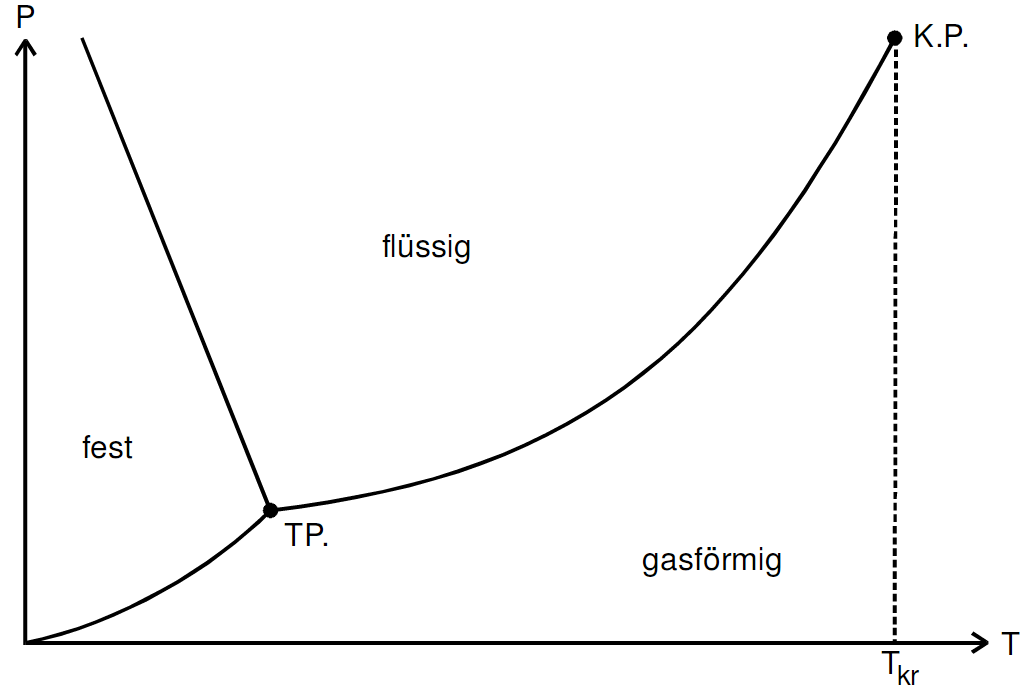
\includegraphics[width=\linewidth-150pt,height=\textheight-150pt,keepaspectratio]{content/Bilder/zustand.png}
	\caption{Eine qualitative Darstellung der einzelnen Aggregatzustände von Wasser\cite{V203}.}
	\label{fig:diagram}
\end{figure}
  Das Verhalten des Stoffes hängt nun von den $P$ und $T$ Parametern ab.
  In den Bereichen der einzelnen Aggregatzustände können alle $P$ und $T$
   Kombinationen des jeweiligen Bereiches erreicht werden ohne das es zu Änderungen kommt.
    Auf den einzelnen Grenzlinien kommt es hingegen zu einer Koexistenz beider
    Aggregatzustände, dass heißt es liegen Teilchen in beiden Zuständen vor.
    Dementsprechend hat das System auf diesen Linien nur noch einen Freiheitsgrad.
    Am Knotenpunkt aller Grenzlinien koexistieren zuletzt Teilchen aller Drei
     Zustände. Diese sind fest bestimmt.

     Es wird sich nun auf die Grenzlinie zwischen flüssigem und gasförmigem Zustand
      beschränkt. Diese heißt Dampfdruckkurve wird hauptsächlich durch die
      Verdampfungwärme $L$ festgelegt. Nun ein näherer Blick auf die Vorgänge von
      Verdampfung und Kondensation.
\subsection{Vorgänge bei Verdampfung und Kondensation}
Wird eine Flüssigkeit in ein evakuiertes Gefäß gefüllt, so kommt es zu einer
 Erhöhung des Druckes im Raum über der Flüssigkeit. Dies folgt, da ein Teil der
  Flüssigkeit in den gasförmigen Zustand wechselt. Die hierfür notwendige
   Energie muss entweder extern hinzugefügt werden oder sie wird der übrigen
    Flüssigkeit in Form eines Temperaturverlustes entnommen. Umgekehrt wird
     Energie bei Rückwechsel in den flüssigen Zustand wieder hinzugefügt. Es
      zeigt sich also ein Kreislauf. Nach hinreichend langer Zeit stellt sich
       ein Gleichgewicht zwischen Dampf und Flüssigkeit ein. Dieser
        Sättigungsdampfdruck hängt von der Temperatur ab und ist invariant unter einer Volumenänderung. Bei letzterer
         verdampft oder kondensiert die nötige Flüssigkeitsmenge.
         \begin{figure}
         	\centering
         	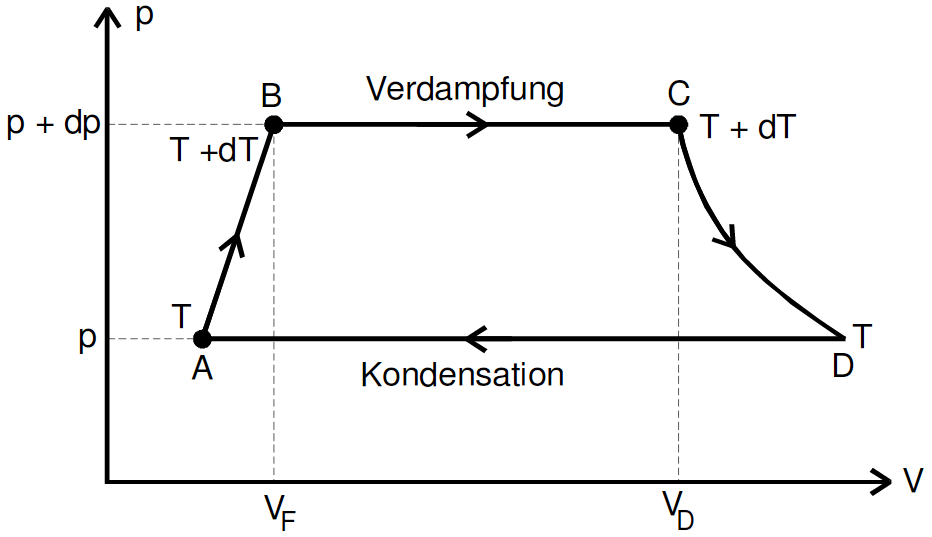
\includegraphics[width=\linewidth-150pt,height=\textheight-150pt,keepaspectratio]{content/Bilder/Kreislauf.png}
         	\caption{Eine mathematische Hilfsskizze zur Ermittlung der Funktion des Druckes auf der Verdampfungskurve\cite{V203}.}
         	\label{fig:Kreislauf}
         \end{figure}
         Stellt man den Kreisprozess nach Abb. \ref{fig:Kreislauf} nun mathematisch da, folgt die Clausius-Clapeyronsche Gleichung:
         \subsection{Lösung der Clausius-Clapeyonschen Gleichung}
         \begin{equation}
           (V_\text{D}-V_\text{F}\text{d}p = \frac{L}{T}\text{d}T \label{eq:DGL}
           \end{equation}
           mit dem Flüssigkeitsvolumen $V_\text{F}$ und dem Dampfvolumen $V_\text{D}$.
Diese lässt sich zunächst nur mit Schwierigkeiten lösen.
Unter den Vereinfachungen:
\begin{itemize}
  \item $V_\text{F}$ ist zuvernachlässigbar klein gegenüber $V_\text{D}$.
  \item $V_\text{D}$ genügt der allgemeinen Gasgleichung $V_\text{D}(p,T) = R\frac{T}{p}$.
  \item Die molare Verdampfungswärme wird als konstant angenommen.
\end{itemize}
lässt sich jedoch eine einfache Lösung. Damit folgt für den Druck auf der Verdampfungskurve:
\begin{equation}
  p = p_0 exp\left(-\frac{L}{RT}\right) \label{eq:DGLLs}
\end{equation}
